\subsection{Aufgabenstellung}
In Anbetracht der Vorteile von Stud.IP, wo bereits eine Struktur installiert ist, welche die Authentifizierung von Benutzern verwaltet und deren Kommunikation ermöglicht, wird die Softwareanwendung als Stud.IP-Plugin entwickelt, das der Plattform hinzugefügt wird und von Benutzern je nach Rolle verwendet werden kann: Student oder Lehrende. Diese Rollen kann man mit StudIP als Tutor oder Dozent modulieren.\\

Für Benutzer mit einer Student-Rolle wird eine Übersicht erstellt, in der sie abhängig von den ausgewählten Auswahlkriterien nach Abschlussarbeiten suchen können.

Benutzer mit einer Lehrende-Rolle verfügen über eine Übersicht, in der sie Abschlussarbeitsthemen hinzufügen, ändern oder löschen können.

\subsubsection{Vorläufige Datenstruktur}
Eine Fakultät kann mehrere Departments haben, jedes Department kann aber nur zu einer Fakultät gehören und es kann verschiedene Fachrichtungen besitzen.
Jede Fachrichtung kann nur zu einem Department zugeordnet werden und kann in mehrere Abteilungen unterteilt werden, wobei eine Abteilung nur zu einer Fachrichtung gehören kann.
Mehrere Betreuer können einer Abteilung zugehörig sein aber ein Betreuer ist jeweils nur einer Abteilung zugeordnet.\\

Ein Thema besteht aus einem Identifikator, einem Namen, einer Beschreibung und ein Veröffentlichungsdatum. Es wird in einer Sprache geschrieben und wird einer Forschungsart zugeordnet: praktisch oder theoretisch. Ebenso besitzt das Thema einen Wert für den Status, wie zum Beispiel reserviert oder in Bearbeitung. Au{ss}erdem werden für das Thema verschiedenen Kompetenzen vorausgesetzt, welche wiederum Voraussetzungen mehrerer Themen sein können.\\
Sollte sich eine Studierende für ein Thema interessieren, kann sie es reservieren. Daraufhin kann ihr das Thema von einem Lehrenden zugeordnet werden.\\

Die vorläufige Entitäten und ihren Beziehungen werden in folgender Abbildung vorgestellt:\\


\cleardoublepage
\begin{figure}[hp]%[H]
    \centering
    %\textbf{Your title}\par\medskip
    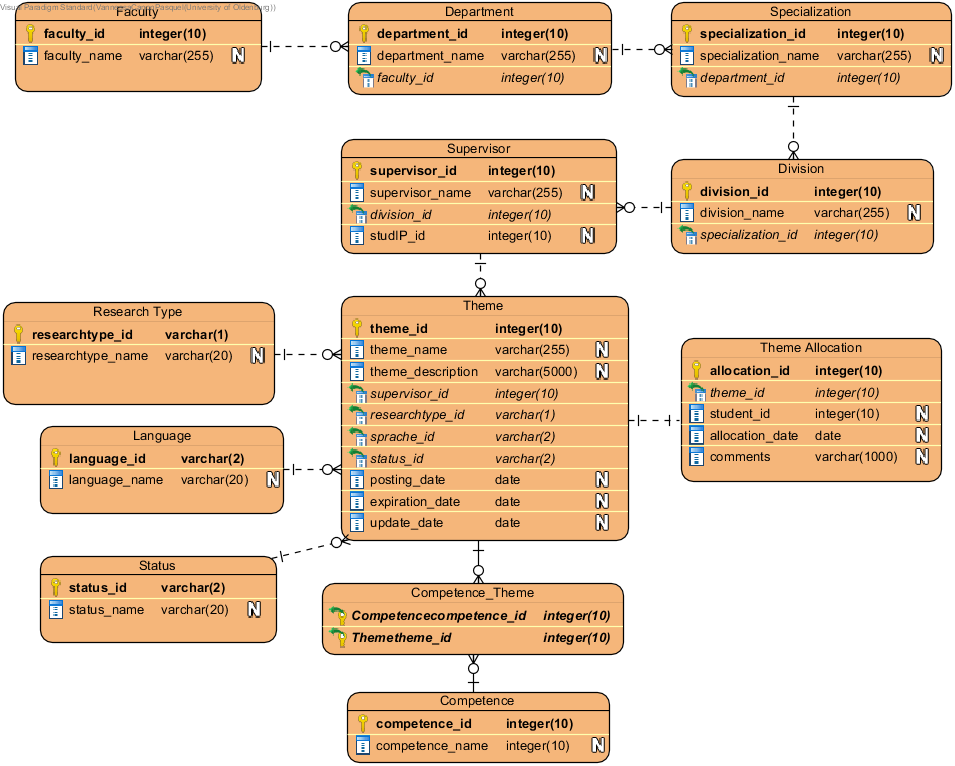
\includegraphics[height=12.5cm,keepaspectratio]{pics/ER_model}\\
    \caption{ER-Modell}
\end{figure}


\subsubsection{Definition von Suchkriterien}
Damit die Ergebnisse den Erwartungen der Studierenden so genau wie möglich entsprechen, wird eine Umfrage auf Basis der vorläufigen Datenstruktur durchgeführt.
In der Umfrage wird gefragt, welche Kriterien sind für die Studierenden relevant, wenn sie nach Themen für Abschlussarbeiten suchen und auch welche zusätzliche Funktionalitäten wären für die Softwareanwendung gewünscht.\\

\newpage
\textbf{Vorläufige Umfrage:}\\

Welche Kriterien sind für Sie relevant, bei der Suche nach Themen für Abschlussarbeiten:
	
	\begin{itemize}
	\item Studienabschluss
	\item Studiengang
	\item Fakultät
		\begin{itemize}[noitemsep]
			\item Department / Institut
			\item Fachrichtung
			\item Abteilung
			\item Betreuer
		\end{itemize}
	\item Forschungsart: Theoretisch, Praktisch
	\item Projekte ansehen
		\begin{itemize}[noitemsep]
			\item Verfügbare
			\item Reservierte
			\item Abgeschlossene
		\end{itemize}
	\item Angeforderte Kompetenzen: JAVA, SQL, Android, IoT, ERP{...}
	\item Sprache
	\item Veröffentlichungsdatum von - bis
	%\item Ähnliche Projekte
	\item Andere:
	\end{itemize}
Gewünschte Funktionalitäten:
	
	\begin{itemize}
	\item Ansprechpartner kontaktieren
	\item Projekt als Favorit merken
	\item Thema reservieren/befreien
	\begin{itemize}[noitemsep]
		\item Mehrere Projekte reservieren
		\item Projekte können von mehreren Studierenden reserviert werden
	\end{itemize}
	\item Andere:	
	\end{itemize}

\subsubsection{Entwurf der Softwareanwendung}
Benutzer können nach der Authentifizierung auf Stud.IP auf die Softwareanwendung-Plugin zugreifen.\\
Die Anwendung wird in PHP entwickelt, da dies die Hauptprogrammiersprache von Stud.IP ist.
Die Benutzeroberfläche enthält grafische Steuerelemente wie Button, Dropdown List, Text Box und Check Box, und es wird in ein Suchabschnitt im linken Bereich der Anwendung und ein Anzeigeabschnitt im rechten Bereich unterteilt, in dem die aus der Datenbank erhaltenen Ergebnisse gemä{\ss} den vom Benutzer ausgewählten Kriterien aufgelistet werden. Gruppen können zusammengeklappt und  aufgeklappt werden.\\

Wenn einen der Datensätze selektiert wird, werden zusätzliche Informationen zum ausgewählten Thema angezeigt, sodass der Benutzer das Abschlussarbeitsthema reservieren kann. Der Status des Themas wird in reserviert geändert, wodurch ein Datensatz in der Themenzuordnungstabelle generiert wird.\\
Die ausgewählten Filter, die Anzahl der abgerufenen Datensätze der Abfrage und eine Option zum Sortieren der Ergebnisse werden im Anwendungsheader angezeigt
Paginierung wird am Ende der Seite eingefügt, um eine gro{\ss}e Anzahl von Datensätzen zu unterstützen.\\

Die folgenden Bilder zeigen das vorläufige Design der Suche Übersicht. Anhang A enthält zusätzliche Bilder des Entwurfs nach dem Anwenden von Filtern.

\begin{figure}[hp]%[H]
    \centering
    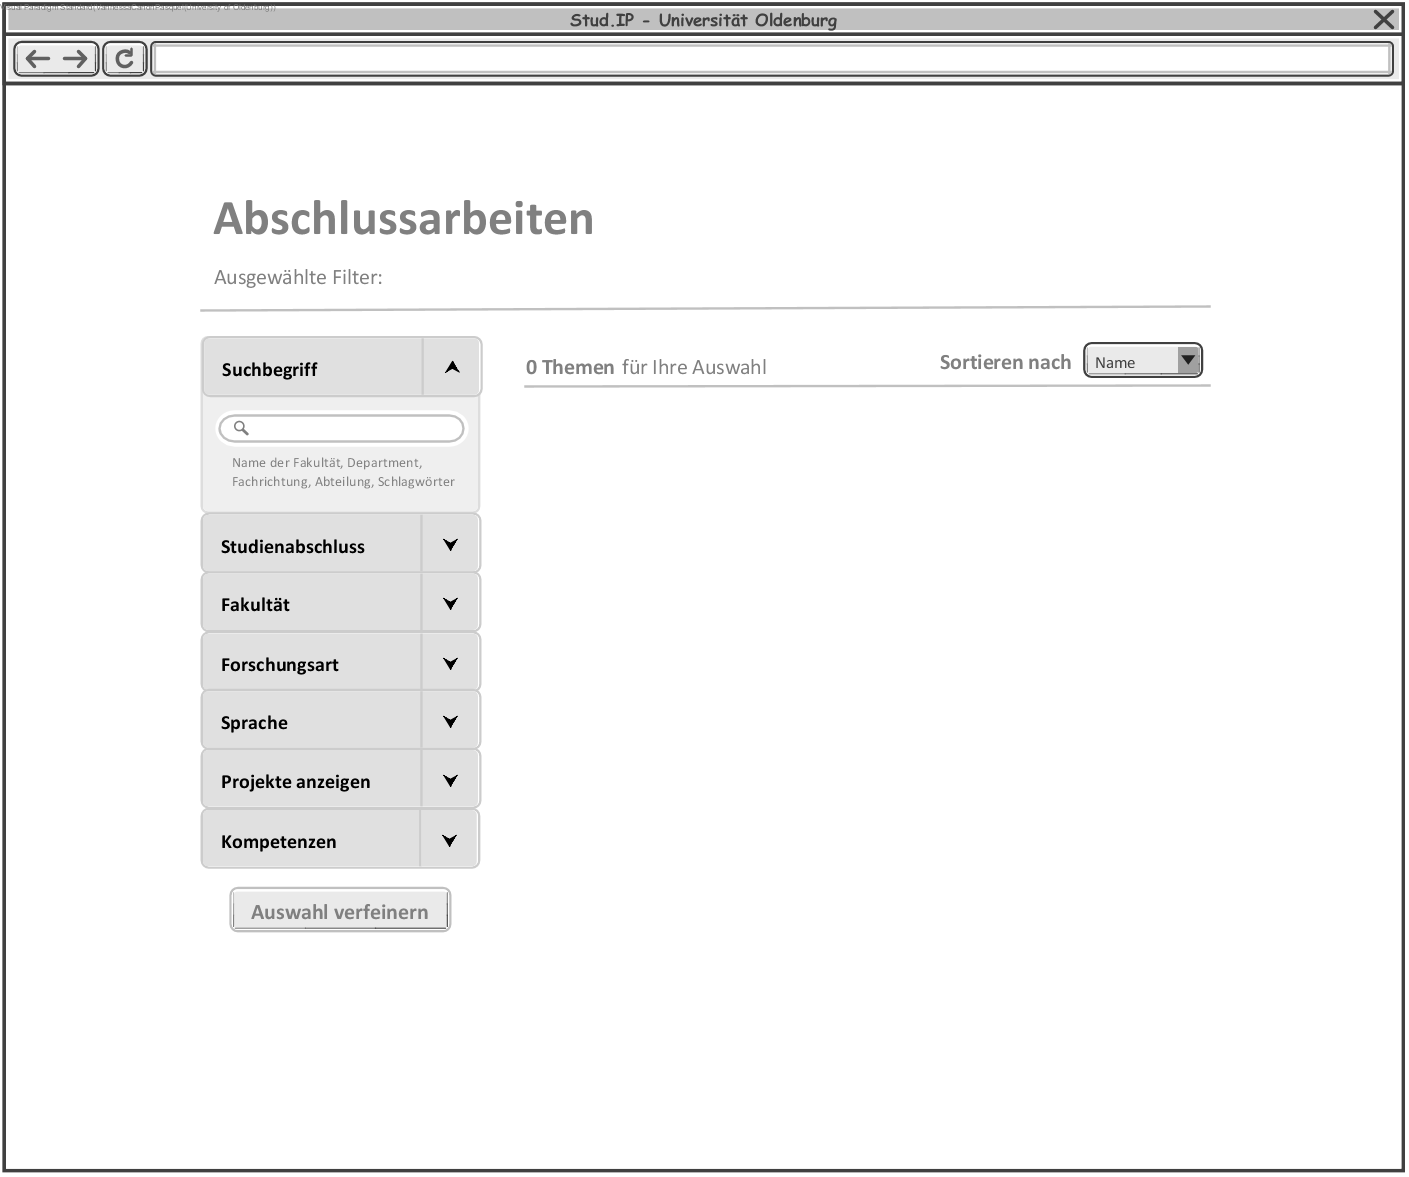
\includegraphics[height=7.5cm,keepaspectratio]{pics/app_collapsed}\\
    \caption{Suchkriterien zusammengeklappt}
\end{figure}

\cleardoublepage
\begin{figure}[hp]%[H]
    \centering
    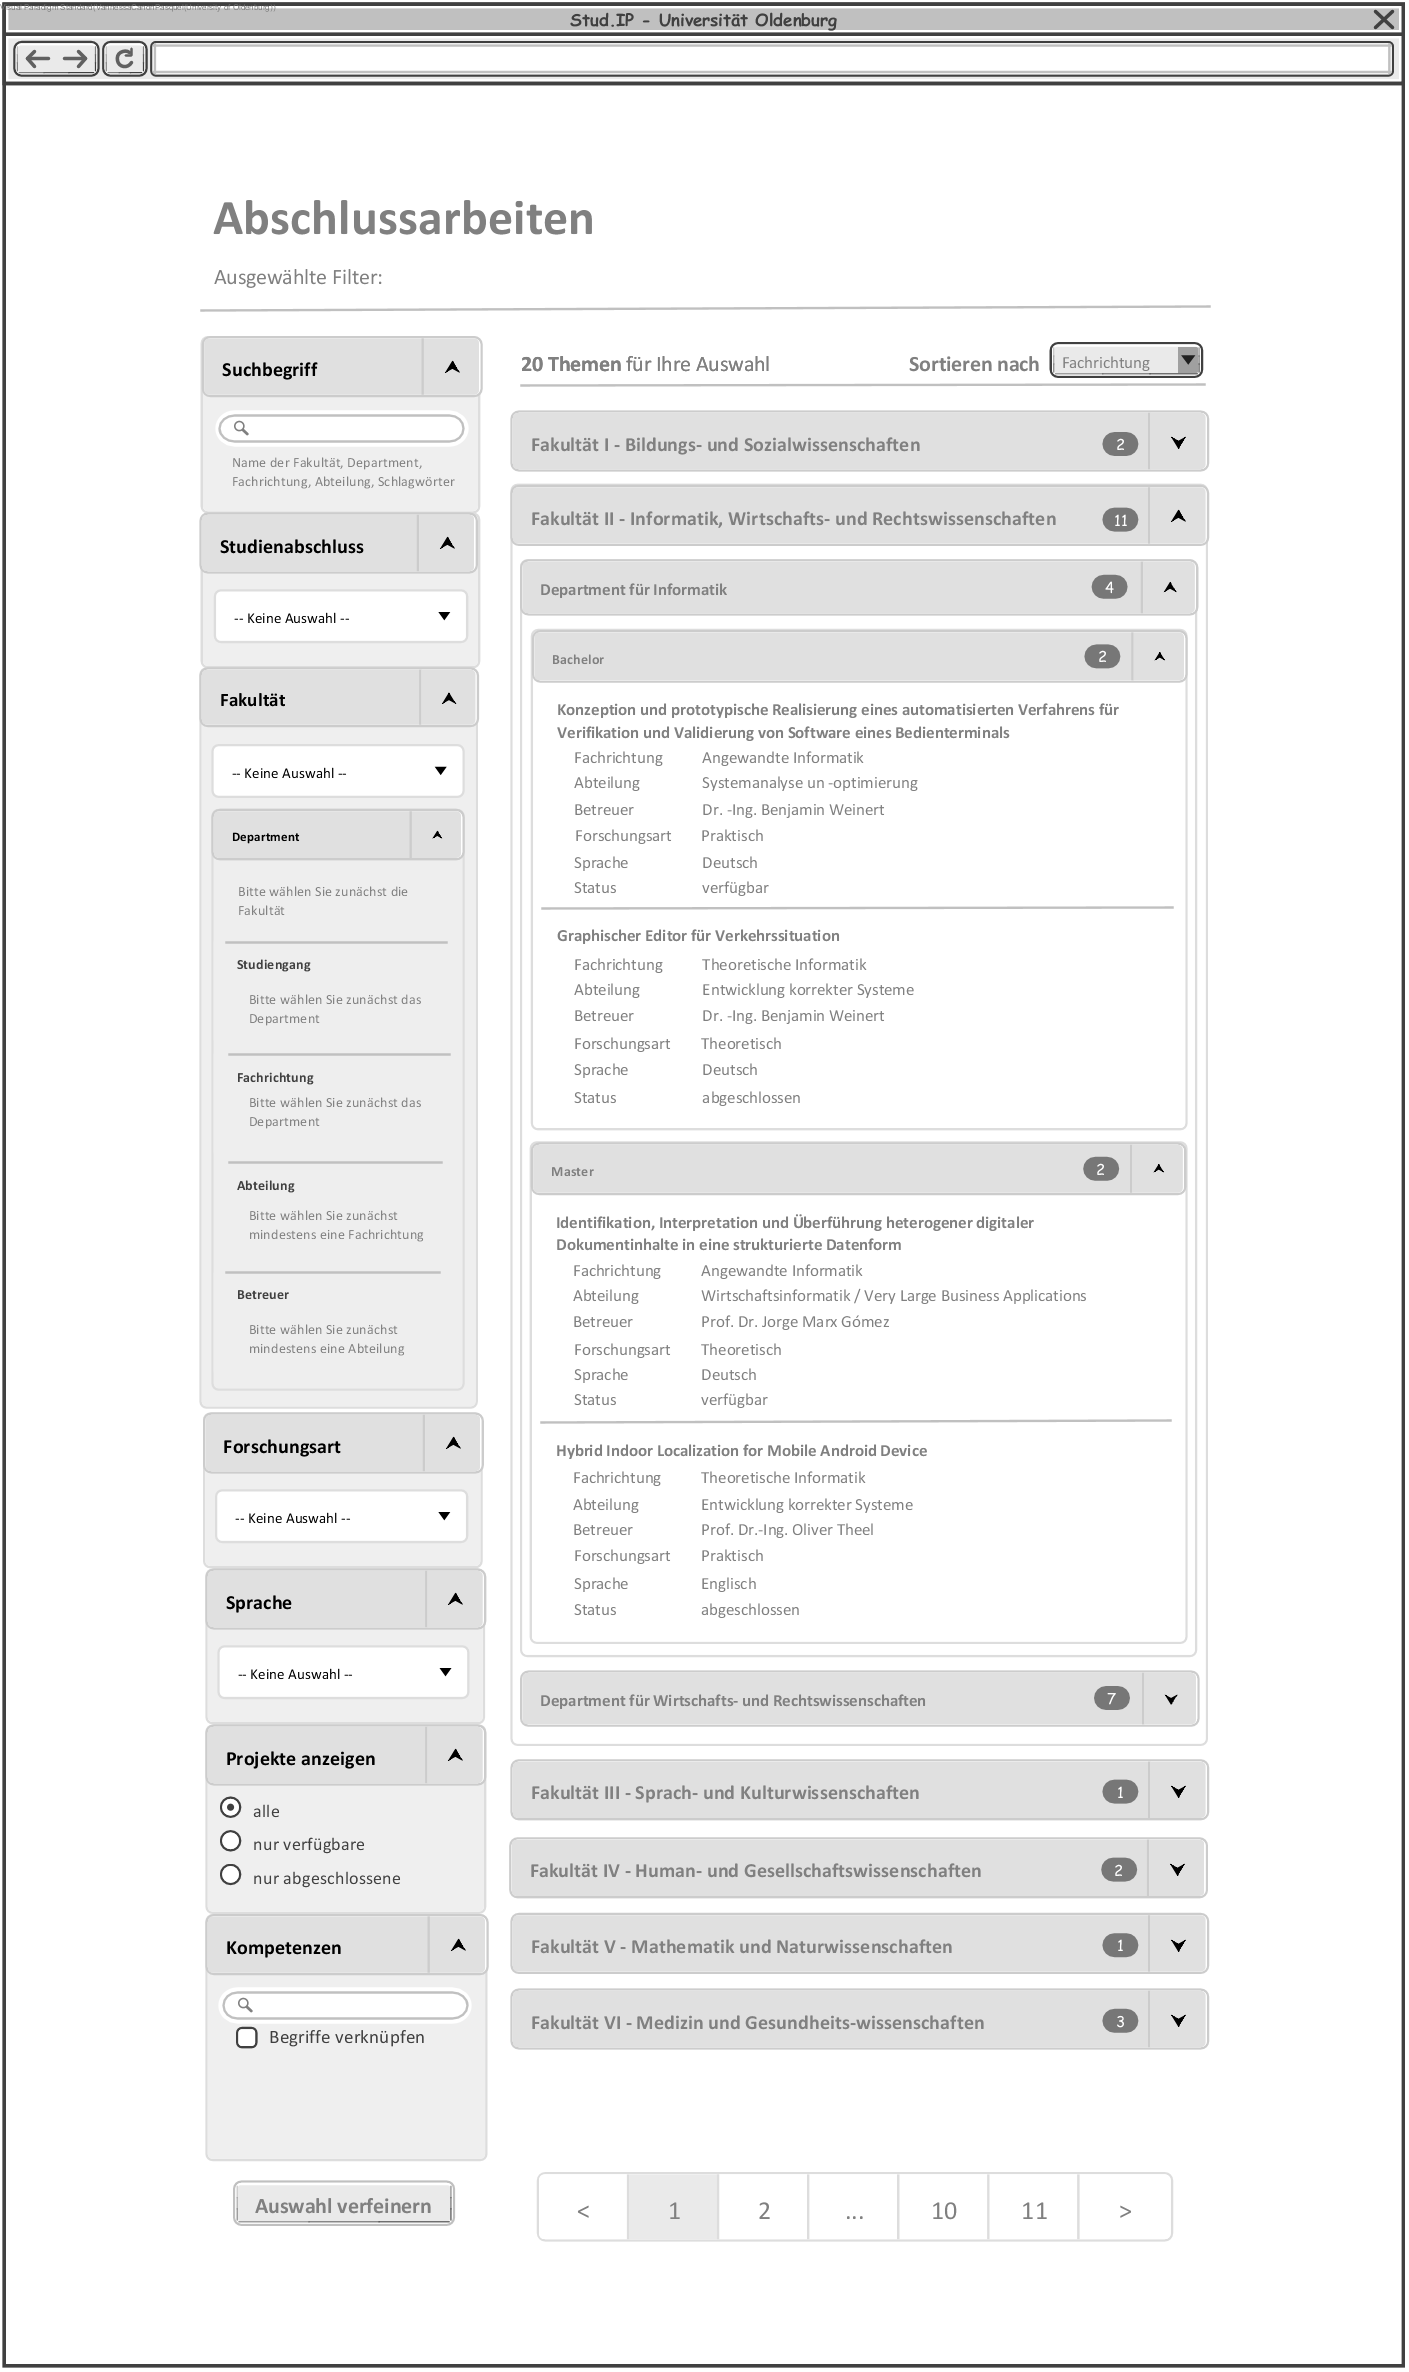
\includegraphics[height=20.5cm,keepaspectratio]{pics/app_expanded}\\
    \caption{Suchkriterien aufgeklappt - ohne Filter}
\end{figure}

\cleardoublepage
Zusätzlich wird eine Grundansicht für die Erstellung, Änderung und Beseitigung von Forschungsthemen durch Benutzer mit einer Lehrende-Rolle hinzugefügt. Dort werden Name, Beschreibung, Forschungsart, Sprache, Status und Ablaufdatum definiert. Nach der Erstellung wird das Veröffentlichungsdatum gespeichert.
Das Forschungsthema wird direkt der Abteilung des Benutzers zugewiesen, es kann jedoch definiert werden, wer der Betreuer ist.\\

Der Benutzer kann den Status des Themas ändern und festlegen, ob er akzeptiert, dass es von mehreren Benutzern reserviert werden kann, falls mehr als ein Benutzer an einem Thema interessiert ist, aber schließlich nur einer von ihnen es annehmen möchte. Ein Thema kann nur einem Benutzer zugewiesen werden.
Nachdem ein Thema geändert wurde, das Aktualisierungsdatum gespeichert.